\documentclass[journal]{IEEEtran}

% *** CITATION PACKAGES ***
%
%\usepackage{cite}
% cite.sty was written by Donald Arseneau
% V1.6 and later of IEEEtran pre-defines the format of the cite.sty package
% \cite{} output to follow that of the IEEE. Loading the cite package will
% result in citation numbers being automatically sorted and properly
% "compressed/ranged". e.g., [1], [9], [2], [7], [5], [6] without using
% cite.sty will become [1], [2], [5]--[7], [9] using cite.sty. cite.sty's
% \cite will automatically add leading space, if needed. Use cite.sty's
% noadjust option (cite.sty V3.8 and later) if you want to turn this off
% such as if a citation ever needs to be enclosed in parenthesis.
% cite.sty is already installed on most LaTeX systems. Be sure and use
% version 5.0 (2009-03-20) and later if using hyperref.sty.
% The latest version can be obtained at:
% http://www.ctan.org/pkg/cite
% The documentation is contained in the cite.sty file itself.






% *** GRAPHICS RELATED PACKAGES ***
%
\ifCLASSINFOpdf
  \usepackage[pdftex]{graphicx}
  % declare the path(s) where your graphic files are
  \graphicspath{{./Figures/}{./photos/}}
  % and their extensions so you won't have to specify these with
  % every instance of \includegraphics
  \DeclareGraphicsExtensions{.pdf,.png}
\else
  % or other class option (dvipsone, dvipdf, if not using dvips). graphicx
  % will default to the driver specified in the system graphics.cfg if no
  % driver is specified.
  \usepackage[dvips]{graphicx}
  % declare the path(s) where your graphic files are
  \graphicspath{{./Figures/}{./photos/}}
  % and their extensions so you won't have to specify these with
  % every instance of \includegraphics
  \DeclareGraphicsExtensions{.pdf,.png}
\fi

% *** MATH PACKAGES ***
%
\usepackage{amsmath}
% A popular package from the American Mathematical Society that provides
% many useful and powerful commands for dealing with mathematics.
%
% Note that the amsmath package sets \interdisplaylinepenalty to 10000
% thus preventing page breaks from occurring within multiline equations. Use:
%\interdisplaylinepenalty=2500
% after loading amsmath to restore such page breaks as IEEEtran.cls normally
% does. amsmath.sty is already installed on most LaTeX systems. The latest
% version and documentation can be obtained at:
% http://www.ctan.org/pkg/amsmath





% *** SPECIALIZED LIST PACKAGES ***
%
%\usepackage{algorithmic}
% algorithmic.sty was written by Peter Williams and Rogerio Brito.
% This package provides an algorithmic environment fo describing algorithms.
% You can use the algorithmic environment in-text or within a figure
% environment to provide for a floating algorithm. Do NOT use the algorithm
% floating environment provided by algorithm.sty (by the same authors) or
% algorithm2e.sty (by Christophe Fiorio) as the IEEE does not use dedicated
% algorithm float types and packages that provide these will not provide
% correct IEEE style captions. The latest version and documentation of
% algorithmic.sty can be obtained at:
% http://www.ctan.org/pkg/algorithms
% Also of interest may be the (relatively newer and more customizable)
% algorithmicx.sty package by Szasz Janos:
% http://www.ctan.org/pkg/algorithmicx




% *** ALIGNMENT PACKAGES ***
%
%\usepackage{array}
% Frank Mittelbach's and David Carlisle's array.sty patches and improves
% the standard LaTeX2e array and tabular environments to provide better
% appearance and additional user controls. As the default LaTeX2e table
% generation code is lacking to the point of almost being broken with
% respect to the quality of the end results, all users are strongly
% advised to use an enhanced (at the very least that provided by array.sty)
% set of table tools. array.sty is already installed on most systems. The
% latest version and documentation can be obtained at:
% http://www.ctan.org/pkg/array


% IEEEtran contains the IEEEeqnarray family of commands that can be used to
% generate multiline equations as well as matrices, tables, etc., of high
% quality.




% *** SUBFIGURE PACKAGES ***
\ifCLASSOPTIONcompsoc
 \usepackage[caption=false,font=normalsize,labelfont=sf,textfont=sf]{subfig}
\else
 \usepackage[caption=false,font=footnotesize]{subfig}
\fi
% subfig.sty, written by Steven Douglas Cochran, is the modern replacement
% for subfigure.sty, the latter of which is no longer maintained and is
% incompatible with some LaTeX packages including fixltx2e. However,
% subfig.sty requires and automatically loads Axel Sommerfeldt's caption.sty
% which will override IEEEtran.cls' handling of captions and this will result
% in non-IEEE style figure/table captions. To prevent this problem, be sure
% and invoke subfig.sty's "caption=false" package option (available since
% subfig.sty version 1.3, 2005/06/28) as this is will preserve IEEEtran.cls
% handling of captions.
% Note that the Computer Society format requires a larger sans serif font
% than the serif footnote size font used in traditional IEEE formatting
% and thus the need to invoke different subfig.sty package options depending
% on whether compsoc mode has been enabled.
%
% The latest version and documentation of subfig.sty can be obtained at:
% http://www.ctan.org/pkg/subfig




% *** FLOAT PACKAGES ***
%
%\usepackage{fixltx2e}
% fixltx2e, the successor to the earlier fix2col.sty, was written by
% Frank Mittelbach and David Carlisle. This package corrects a few problems
% in the LaTeX2e kernel, the most notable of which is that in current
% LaTeX2e releases, the ordering of single and double column floats is not
% guaranteed to be preserved. Thus, an unpatched LaTeX2e can allow a
% single column figure to be placed prior to an earlier double column
% figure.
% Be aware that LaTeX2e kernels dated 2015 and later have fixltx2e.sty's
% corrections already built into the system in which case a warning will
% be issued if an attempt is made to load fixltx2e.sty as it is no longer
% needed.
% The latest version and documentation can be found at:
% http://www.ctan.org/pkg/fixltx2e


%\usepackage{stfloats}
% stfloats.sty was written by Sigitas Tolusis. This package gives LaTeX2e
% the ability to do double column floats at the bottom of the page as well
% as the top. (e.g., "\begin{figure*}[!b]" is not normally possible in
% LaTeX2e). It also provides a command:
%\fnbelowfloat
% to enable the placement of footnotes below bottom floats (the standard
% LaTeX2e kernel puts them above bottom floats). This is an invasive package
% which rewrites many portions of the LaTeX2e float routines. It may not work
% with other packages that modify the LaTeX2e float routines. The latest
% version and documentation can be obtained at:
% http://www.ctan.org/pkg/stfloats
% Do not use the stfloats baselinefloat ability as the IEEE does not allow
% \baselineskip to stretch. Authors submitting work to the IEEE should note
% that the IEEE rarely uses double column equations and that authors should try
% to avoid such use. Do not be tempted to use the cuted.sty or midfloat.sty
% packages (also by Sigitas Tolusis) as the IEEE does not format its papers in
% such ways.
% Do not attempt to use stfloats with fixltx2e as they are incompatible.
% Instead, use Morten Hogholm'a dblfloatfix which combines the features
% of both fixltx2e and stfloats:
%
\usepackage{dblfloatfix}
% The latest version can be found at:
% http://www.ctan.org/pkg/dblfloatfix




%\ifCLASSOPTIONcaptionsoff
%  \usepackage[nomarkers]{endfloat}
% \let\MYoriglatexcaption\caption
% \renewcommand{\caption}[2][\relax]{\MYoriglatexcaption[#2]{#2}}
%\fi
% endfloat.sty was written by James Darrell McCauley, Jeff Goldberg and 
% Axel Sommerfeldt. This package may be useful when used in conjunction with 
% IEEEtran.cls'  captionsoff option. Some IEEE journals/societies require that
% submissions have lists of figures/tables at the end of the paper and that
% figures/tables without any captions are placed on a page by themselves at
% the end of the document. If needed, the draftcls IEEEtran class option or
% \CLASSINPUTbaselinestretch interface can be used to increase the line
% spacing as well. Be sure and use the nomarkers option of endfloat to
% prevent endfloat from "marking" where the figures would have been placed
% in the text. The two hack lines of code above are a slight modification of
% that suggested by in the endfloat docs (section 8.4.1) to ensure that
% the full captions always appear in the list of figures/tables - even if
% the user used the short optional argument of \caption[]{}.
% IEEE papers do not typically make use of \caption[]'s optional argument,
% so this should not be an issue. A similar trick can be used to disable
% captions of packages such as subfig.sty that lack options to turn off
% the subcaptions:
% For subfig.sty:
% \let\MYorigsubfloat\subfloat
% \renewcommand{\subfloat}[2][\relax]{\MYorigsubfloat[]{#2}}
% However, the above trick will not work if both optional arguments of
% the \subfloat command are used. Furthermore, there needs to be a
% description of each subfigure *somewhere* and endfloat does not add
% subfigure captions to its list of figures. Thus, the best approach is to
% avoid the use of subfigure captions (many IEEE journals avoid them anyway)
% and instead reference/explain all the subfigures within the main caption.
% The latest version of endfloat.sty and its documentation can obtained at:
% http://www.ctan.org/pkg/endfloat
%
% The IEEEtran \ifCLASSOPTIONcaptionsoff conditional can also be used
% later in the document, say, to conditionally put the References on a 
% page by themselves.




% *** PDF, URL AND HYPERLINK PACKAGES ***
%
\usepackage{url}
% url.sty was written by Donald Arseneau. It provides better support for
% handling and breaking URLs. url.sty is already installed on most LaTeX
% systems. The latest version and documentation can be obtained at:
% http://www.ctan.org/pkg/url
% Basically, \url{my_url_here}.




% *** Do not adjust lengths that control margins, column widths, etc. ***
% *** Do not use packages that alter fonts (such as pslatex).         ***
% There should be no need to do such things with IEEEtran.cls V1.6 and later.
% (Unless specifically asked to do so by the journal or conference you plan
% to submit to, of course. )


% correct bad hyphenation here
\hyphenation{op-tical net-works semi-conduc-tor}

% *** Math formatting
\usepackage{amsfonts}

% *** Equalize bottom
\usepackage{flushend}

% *** Include Code
\usepackage{listings}

% *** Custom definitions
\newcommand{\R}{\mathbb{R}}
\newcommand{\N}{\mathcal{N}}
\newcommand{\I}{\mathbb{I}}
\newcommand{\II}{\mathbb{II}}
\newcommand{\Shape}{\mathcal{S}}
\newcommand{\Z}{\mathbb{Z}}
\newcommand\given[1][]{\:#1\vert\:}


\begin{document}
%
% paper title
% Titles are generally capitalized except for words such as a, an, and, as,
% at, but, by, for, in, nor, of, on, or, the, to and up, which are usually
% not capitalized unless they are the first or last word of the title.
% Linebreaks \\ can be used within to get better formatting as desired.
% Do not put math or special symbols in the title.
\title{Sphere Under Advection and Mean Curvature Flow}
%
%
% author names and IEEE memberships
% note positions of commas and nonbreaking spaces ( ~ ) LaTeX will not break
% a structure at a ~ so this keeps an author's name from being broken across
% two lines.
% use \thanks{} to gain access to the first footnote area
% a separate \thanks must be used for each paragraph as LaTeX2e's \thanks
% was not built to handle multiple paragraphs
%

% \IEEEauthorblockN{
%   Bryce~A~Besler\IEEEauthorrefmark{1}, 
%   Tannis~D~Kemp\IEEEauthorrefmark{1}, 
%   Nils~D~Forkert\IEEEauthorrefmark{2}\IEEEauthorrefmark{3}, 
%   Steven~K~Boyd\IEEEauthorrefmark{1}\IEEEauthorrefmark{3},
% } \\
% \IEEEauthorblockA{
%   \IEEEauthorrefmark{1}McCaig Institute for Bone and Joint Health
% } \\
% \IEEEauthorblockA{
%   \IEEEauthorrefmark{2}Hotchkiss Brain Institute
% } \\
% \IEEEauthorblockA{
%   \IEEEauthorrefmark{3}Department of Radiology
% }\\
% University of Calgary, Canada

\author{
  Bryce~A.~Besler,
  Tannis~D.~Kemp,
  Nils~D.~Forkert,
  Steven~K.~Boyd

\thanks{This work was supported by the Natural Sciences and Engineering Research Council (NSERC) of Canada, grant RGPIN-2019-04135.}
\thanks{B.A. Besler and T. D. Kemp are in the McCaig Institute for Bone and Joint Health, University of Calgary Canada. N.D. Forkert is with the Department of Radiology and the Hotchkiss Brain Institute, University of Calgary, Canada. S.K. Boyd is with the Department of Radiology and McCaig Institute for Bone and Joint Health, University of Calgary Canada e-mail: skboyd@ucalgary.ca}% <-this % stops a space
}

% note the % following the last \IEEEmembership and also \thanks - 
% these prevent an unwanted space from occurring between the last author name
% and the end of the author line. i.e., if you had this:
% 
% \author{....lastname \thanks{...} \thanks{...} }
%                     ^------------^------------^----Do not want these spaces!
%
% a space would be appended to the last name and could cause every name on that
% line to be shifted left slightly. This is one of those "LaTeX things". For
% instance, "\textbf{A} \textbf{B}" will typeset as "A B" not "AB". To get
% "AB" then you have to do: "\textbf{A}\textbf{B}"
% \thanks is no different in this regard, so shield the last } of each \thanks
% that ends a line with a % and do not let a space in before the next \thanks.
% Spaces after \IEEEmembership other than the last one are OK (and needed) as
% you are supposed to have spaces between the names. For what it is worth,
% this is a minor point as most people would not even notice if the said evil
% space somehow managed to creep in.


% The paper headers
\markboth{}%
{Besler \MakeLowercase{\textit{et al.}}: Sphere under Advection and Mean Curvature Flow}
% The only time the second header will appear is for the odd numbered pages
% after the title page when using the twoside option.
% 
% *** Note that you probably will NOT want to include the author's ***
% *** name in the headers of peer review papers.                   ***
% You can use \ifCLASSOPTIONpeerreview for conditional compilation here if
% you desire.




% If you want to put a publisher's ID mark on the page you can do it like
% this:
%\IEEEpubid{0000--0000/00\$00.00~\copyright~2015 IEEE}
% Remember, if you use this you must call \IEEEpubidadjcol in the second
% column for its text to clear the IEEEpubid mark.



% use for special paper notices
%\IEEEspecialpapernotice{(Invited Paper)}




% make the title area
\maketitle

% As a general rule, do not put math, special symbols or citations
% in the abstract or keywords.
\begin{abstract}
Advection and mean curvature flow is used as a model of bone microarchitecture adaptation.
It is an equivalent geometric flow to prescribed mean curvature flow with an additional rate term.
In order to validate numerical methods for simulating this flow and developing an inverse solver, a closed-form solution for advection and mean curvature flow of a sphere is derived.
\end{abstract}

% Note that keywords are not normally used for peerreview papers.
\begin{IEEEkeywords}
Geometric Flow, Mean Curvature, Advection
\end{IEEEkeywords}

\section{Introduction}
Advection and mean curvature flow has recently been used as a model for predicting bone microarchitecture changes during aging~\cite{besler2018bone}.
Towards validating numerical solver and inverse problems therein, a closed-form solution to advection and mean curvature flow of a sphere is sought.
The contents of this article are largely pedagogical.

\section{Advection and Mean Curvature Flow}
Consider an orientable, closed two-dimensional surface immersed in three dimensions $M \colon \!R^2 \rightarrow \!R^3$ with mean curvature $\kappa$ and unit normal $\hat{n}$.
A combination of advection and mean curvature flow is considered where the advection is given by a scalar rate $a$ along the unit normal direction and mean curvature is given by a rate constant $b$.
\begin{equation}
  \label{eqn:advection-mean}
  \frac{\partial M}{\partial t} = (a - b \kappa) \hat{n}
\end{equation}

Such a flow is equivalent to flow under prescribed mean curvature with an additional rate term:
\begin{equation}
  \frac{\partial M}{\partial t} = b(\tilde{\kappa} - \kappa) \hat{n}
\end{equation}
where $\tilde{\kappa} = a/b$ is the prescribed mean curvature.
The study of this flow originates from the geometric similarities between triply period minimal surfaces~\cite{schoen1970infinite,anderson1987periodic,chopp1993flow} and bone microarchitecture~\cite{hildebrand1999direct}.
It should be noted that $\tilde{\kappa}$ is not the total mean curvature and that this is not a volume preserving flow.
More precisely, the flow permits the development of singularities, producing a change in topology.

In general, $a$ can be any real number while $b$ should be a real number greater than or equal to zero.
A negative value for $b$ would imply inverse mean curvature flow, which is unstable when points on the surface have zero mean curvature.
One can see that the flow stops when $\kappa = \tilde{\kappa} = a/b$ everywhere on the surface.

\section{The Sphere}
This paper is concerned with a closed-form solution to a sphere moving under advection and mean curvature.
All work will be done on the two-sphere $S_2$.

Consider the two-sphere mapping to spherical coordinates $M \colon (u,v) \rightarrow (\rho, \theta, \phi)$ with radius $r_0$.
\begin{align}
  \label{eqn:sphere:mapping}
  \begin{pmatrix}
    \rho \\
    \theta \\
    \phi
  \end{pmatrix} = 
  \begin{pmatrix}
    r_0 \cos u \sin v \\
    r_0 \sin u \sin v \\
    r_0 \cos v
  \end{pmatrix}
\end{align}
The normal is along the radial direction.
\begin{equation}
  \label{eqn:sphere:normal}
  \hat{n}(u,v) = 1\hat{\rho} + 0 \hat{u} + 0 \hat{v}
\end{equation}
Since the surface normal is aligned with the $\hat{\rho}$ direction, all curve evolution problems will reduce to a differential equation on the radius by spherical symmetry.
The mean curvature at every point is the inverse of radius.
\begin{equation}
  \label{eqn:sphere:curvature}
  \kappa(u,v) = 1/r
\end{equation}
These prerequisites allow the development of a closed-form solution for the sphere.

\section{Sphere Under Advection}
\label{sec:advection}
Lets begin with the problem of advection ($b = 0$).
In this case, Equation~\ref{eqn:advection-mean} reduces to a simple expression:
\begin{equation}
  \frac{\partial M}{\partial t} = a \hat{n}
\end{equation}
Substituting Equations~\ref{eqn:sphere:mapping} and \ref{eqn:sphere:normal}:
\begin{align}
  \begin{pmatrix}
    \rho_t \\
    \theta_t \\
    \phi_t
  \end{pmatrix} = a \cdot
  \begin{pmatrix}
    1 \cdot \hat{\rho} \\
    0 \cdot \hat{\theta} \\
    0 \cdot \hat{\phi}
  \end{pmatrix}
\end{align}
where $\left(\cdot\right)_t$ is shorthand for a temporal derivative.
This gives a single initial value problem to solve:
\begin{equation}
  \left\{
    \begin{array}{ll}
      \rho_t = a\\
      \rho(0) = r_0
    \end{array}
  \right.
\end{equation}
The solution is immediate:
\begin{equation}
  \label{eqn:advection:solution}
  \rho(t) = r_0 + at
\end{equation}

Equation~\ref{eqn:advection:solution} agrees with intuition.
The surface is moving at a linear rate of $a$ units of distance per units of time along the normal of the sphere.
If $a$ is positive, the sphere grows forever.
If $a$ is negative, it shrinks until it vanishes at the time $t = -r_0/a$.
The solution is plotted for five values of $a$ in Figure~\ref{fig:advection}.

\begin{figure}[t]
  \centering
    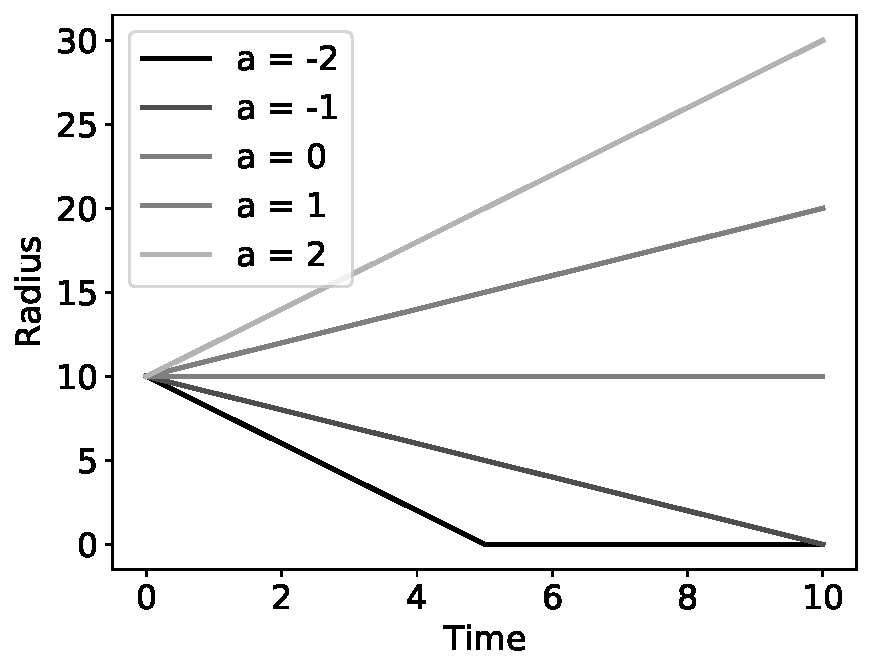
\includegraphics[width=0.9\linewidth]{advection}%
  \caption{Advection solution to the sphere ($r_0 = 10$).}
  \label{fig:advection}
\end{figure}

\section{Sphere Under Mean Curvature Flow}
\label{sec:meanflow}
Attention is now placed on mean curvature flow ($a = 0$).
In this case, Equation~\ref{eqn:advection-mean} reduces to a simple expression:
\begin{equation}
  \label{eqn:mean}
  \frac{\partial M}{\partial t} = -b \kappa \hat{n}
\end{equation}
Substituting Equations~\ref{eqn:sphere:mapping}, \ref{eqn:sphere:normal} and \ref{eqn:sphere:curvature}:
\begin{align}
  \begin{pmatrix}
    \rho_t \\
    \theta_t \\
    \phi_t
  \end{pmatrix} = -b / \rho \cdot
  \begin{pmatrix}
    1 \cdot \hat{\rho} \\
    0 \cdot \hat{\theta} \\
    0 \cdot \hat{\phi}
  \end{pmatrix}
\end{align}
Again, this leads to a single initial value problem:
\begin{equation}
  \left\{
    \begin{array}{ll}
      \rho_t = -b/\rho\\
      \rho(0) = r_0
    \end{array}
  \right.
\end{equation}
Through some substitution, the problem can be solved:
\begin{equation}
  \label{eqn:mean:solution}
  \rho(t) = \sqrt{r_0^2 - 2bt}
\end{equation}
This solution is a classic pedagogical result in mean curvature flow~\cite{bellettini2014lecture}.

As with advection, Equation~\ref{eqn:mean:solution} agrees with intuition.
Since the mean curvature everywhere on a sphere is positive and $b$ is positive, the negative sign in Equation~\ref{eqn:mean} suggests that the sphere is always shrinking.
Indeed, the sphere shrinks until it vanishes at $t = r_0^2/2b$.
The solution is plotted for five values of $b$ in Figure~\ref{fig:mean}.

\begin{figure}[t]
  \centering
    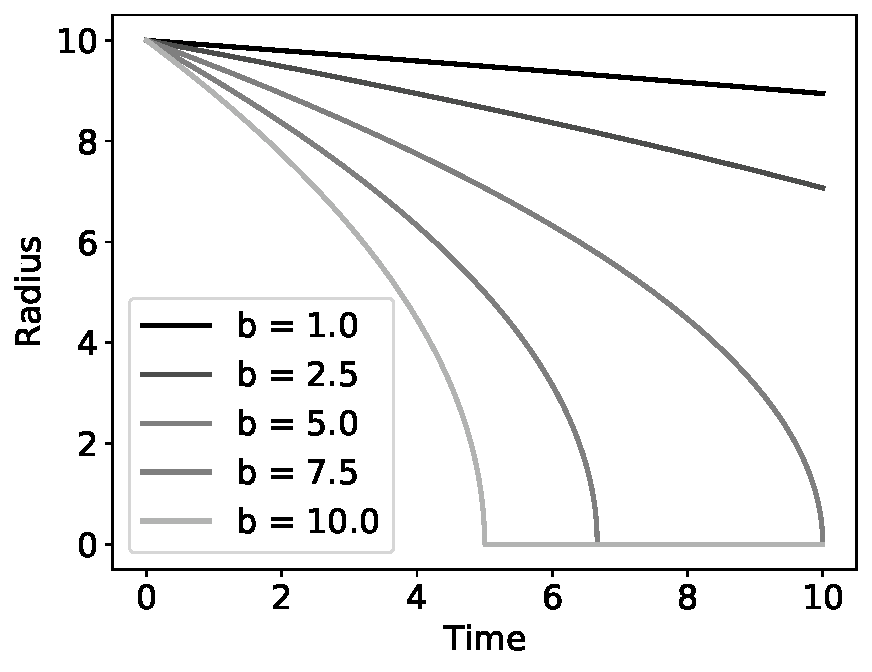
\includegraphics[width=0.9\linewidth]{mean}%
  \caption{Mean curvature solution to the sphere ($r_0 = 10$).}
  \label{fig:mean}
\end{figure}

\section{Sphere Under Advection and Mean Curvature Flow}
Having some background and intuition, the main solution is sought.
Skipping the middle steps as described in Sections~\ref{sec:advection} and \ref{sec:meanflow}, the initial value problem can be stated.
\begin{equation}
  \label{eqn:base}
  \left\{
    \begin{array}{ll}
      r_t = a - \frac{b}{r}\\
      r(0) = r_0
    \end{array}
  \right.
\end{equation}
Notation is changed from $\rho$ to $r$ for ease of interpretation.

Analyzing Equation~\ref{eqn:base} can give insight into the model.
In general, the model stops flowing when $r_t = 0$, which corresponds to $r = b/a$.
However, this is only the case when $a$ is positive.
When $a$ is negative, the sphere shrinks forever.
When $a$ is positive, there exists a point where the shrinking under mean curvature is balanced by the growth from advection.
However, this point is only meta-stable.
If the initial sphere radius is exactly $r_0 = b/a$, the sphere will be constant over time.
However, if the radius is slightly increased, the mean curvature term decreases and the sphere grows.
If the radius is slightly shrunk, the mean curvature term increases and the sphere shrinks.
In summary:
\begin{itemize}
  \item $a < 0 \rightarrow$ shrink to zero
  \item $0 < a < \frac{b}{r_0} \rightarrow $ shrink to zero
  \item $ a = \frac{b}{r_0} \rightarrow $ meta-stable
  \item $\frac{b}{r_0} < a \rightarrow $ grow to infinity
\end{itemize}
In general, away from the meta-stable point, when growing, growth is like advection. When shrinking, shrinking is like mean curvature flow.
This is demonstrated in a phase diagram in Figure~\ref{fig:loss}.

\begin{figure}[b]
  \centering
    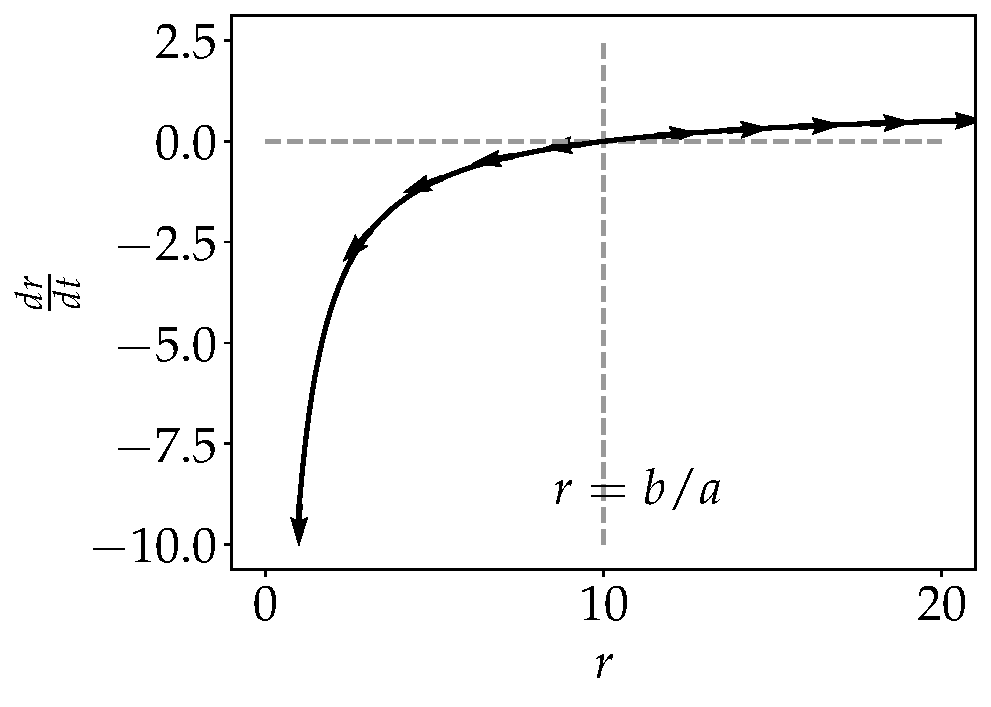
\includegraphics[width=0.9\linewidth]{loss}%
  \caption{Plotting the meta-stable point of the sphere under advection and mean curvature ($a = 1$, $b = 10$).}
  \label{fig:loss}
\end{figure}

Now, the closed-form solution to Equation~\ref{eqn:base} is derived.
\begin{eqnarray}
  \frac{dr}{dt} = a - \frac{b}{r} \\
  \frac{r}{ar - b} dr = dt
\end{eqnarray}
Using the substitution $x = ar-b$ leads to:
\begin{eqnarray}
  \frac{x+b}{a}\frac{1}{x} \frac{dx}{a} = dt \\
  \left[\frac{1}{a^2} + \frac{b}{ax}\right] dx = dt
\end{eqnarray}
Which can be integrated:
\begin{equation}
  \frac{ar-b}{a^2} + \frac{b}{a^2}\ln\left(ar-b\right) = t + c
\end{equation}
It is convenient to solve for $c$ at this point with the initial condition $r(0) = r_0$.
\begin{equation}
  c = \frac{ar_0-b}{a^2} + \frac{b}{a^2}\ln\left(ar_0 - b\right)
\end{equation}
The final step is to solve for $r$.
\begin{eqnarray}
  \label{eqn:near-solved}
  \exp\left( \frac{ar-b}{b}\right) \frac{ar-b}{b} = \frac{1}{b}\exp\left(\frac{a^2}{b}(t+c)\right)
\end{eqnarray}
While this appears unsolvable, the left hand side of Equation~\ref{eqn:near-solved} is known as the ``product log" or Lambert W function~\cite{lambert1758observationes,weisstein2002lambert}.
\begin{eqnarray}
  xe^x &=& z \\
  x &=& W_k(z)
\end{eqnarray}
The Lambert W function is plotted in Figure~\ref{fig:w}.
In the case of Equation~\ref{eqn:near-solved},
\begin{eqnarray}
  \label{eqn:x}
  x &=& \frac{ar-b}{b} \\
  z &=& \frac{1}{b} \exp\left(\frac{a^2}{b}(t+c)\right)
\end{eqnarray}

\begin{figure}[b]
  \centering
    \includegraphics[width=0.9\linewidth]{w}%
  \caption{Plotting the Lambert W function for real numbers.}
  \label{fig:w}
\end{figure}

Using the Lambert W and substituting $c$ allows us to solve for $r$:
\begin{eqnarray}
  \frac{ar-b}{b} = W_k\left(\frac{1}{b}\exp\left(\frac{a^2}{b}(t+c)\right)\right) \\
  \label{eqn:soln}
  r = \frac{b}{a}\left(W_k\left[\frac{ar_0-b}{b} \exp\left(\frac{ar_0-b}{b}\right)\exp\left(\frac{a^2t}{b}\right)\right] + 1\right)
\end{eqnarray}

Next, the appropriate branch of $W_k$ must be selected since multiple solutions are possible.
Since this problem deals with real and not complex numbers, only $W_0$ and $W_{-1}$ are available.
From Figure~\ref{fig:w}, two solutions can be seen for $z < 0$, the solutions changing when $x = -1$.
Using Equation~\ref{eqn:x}, the switching condition can be defined.
\begin{eqnarray}
  \frac{ar-b}{b} < -1 \\
  ar < 0
\end{eqnarray}
However, $r$ is always positive since it is the radius of a sphere.
As such, use $W_{-1}$ if $a<0$ and use $W_0$ if $a>0$.
Note that this piecewise function is continuous at $a=0$.

The final step is to derive a vanishing time for the solution.
Again, the vanishing time is the $t$ when $r(t)=0$, which is when $W_k(z) = -1$.
This corresponds to the situation when the argument of $W_k$ in Equation~\ref{eqn:soln} is equal to $\frac{-1}{e}$.
Looking at that argument, the vanishing time is found.
\begin{eqnarray}
  \frac{ar_0-b}{b} \exp\left(\frac{ar_0-b}{b}\right)\exp\left(\frac{a^2t}{b}\right) = \frac{-1}{e} \\
  \label{eqn:vanish1}
  t = \frac{b}{a^2} \ln\left(\frac{b}{b-ar_0}\right) - \frac{r_0}{a}
\end{eqnarray}
Equation~\ref{eqn:vanish1} will only be valid when the argument to the natural logarithm is positive.
\begin{eqnarray}
  \frac{b}{b-ar_0} > 0 \\
  b - ar_0 > 0 \\
  r_0 < \frac{b}{a}
\end{eqnarray}
This is the same condition that was found earlier from analysis of the differential equation.
The equation for vanishing time is then given:
\begin{equation}
  \label{eqn:vanish}
  t = \left\{
    \begin{matrix}
      \infty & \text{ if } r_0 \geq \frac{b}{a} \\
      \frac{b}{a^2} \ln\left(\frac{b}{b-ar_0}\right) - \frac{r_0}{a} & \text{ if } r_0 < \frac{b}{a}
    \end{matrix}
  \right.
\end{equation}
Taking the limits as $a \rightarrow 0$ or as $b \rightarrow 0$ of Equation~\ref{eqn:vanish}, the advection and mean curvature vanishing times from before can be found.

An implementation of the closed-form solution is given in the Appendix.
To finalize the analysis, the solution is plotted in Figure~\ref{fig:solution} for various parameters.
The solution is only of interest around the meta-stable point.
Outside the meta-stable point, one of the two terms is much smaller than the other, meaning only one term drives the flow.
This is important to consider for inverse solvers which may not be able to accurately solve for the non-dominant parameter in this simple geometry.

\begin{figure}[h]
  \centering
  \begin{tabular}{c}
    \subfloat[$r_0 = 11, a = 1, b = 10$]{
      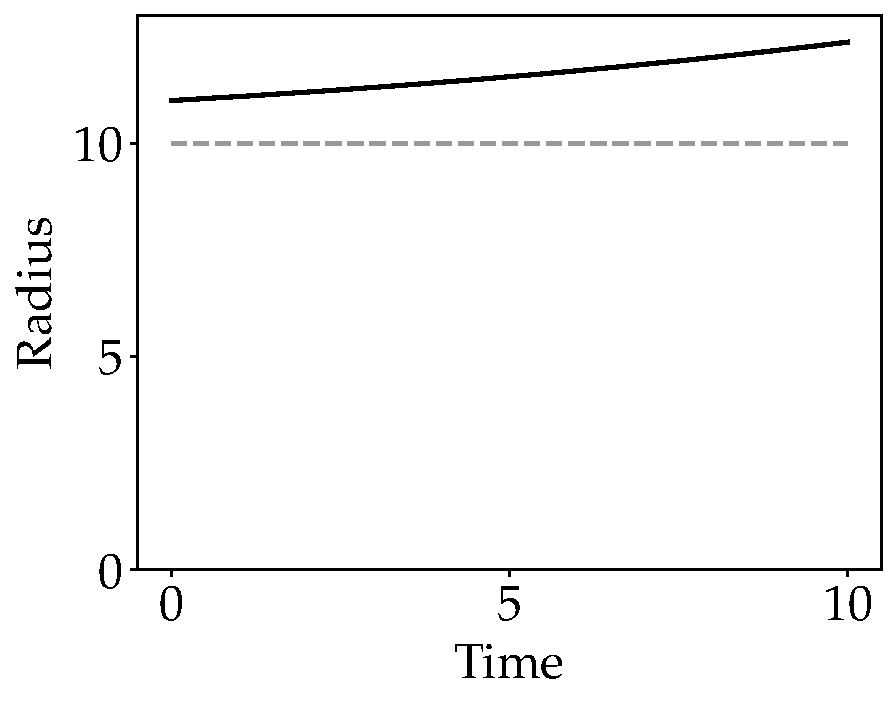
\includegraphics[width=0.85\linewidth]{solution_1}%
      \label{fig:solution:1}
    } \\
    \subfloat[$r_0 = 9, a = 1, b = 10$]{
      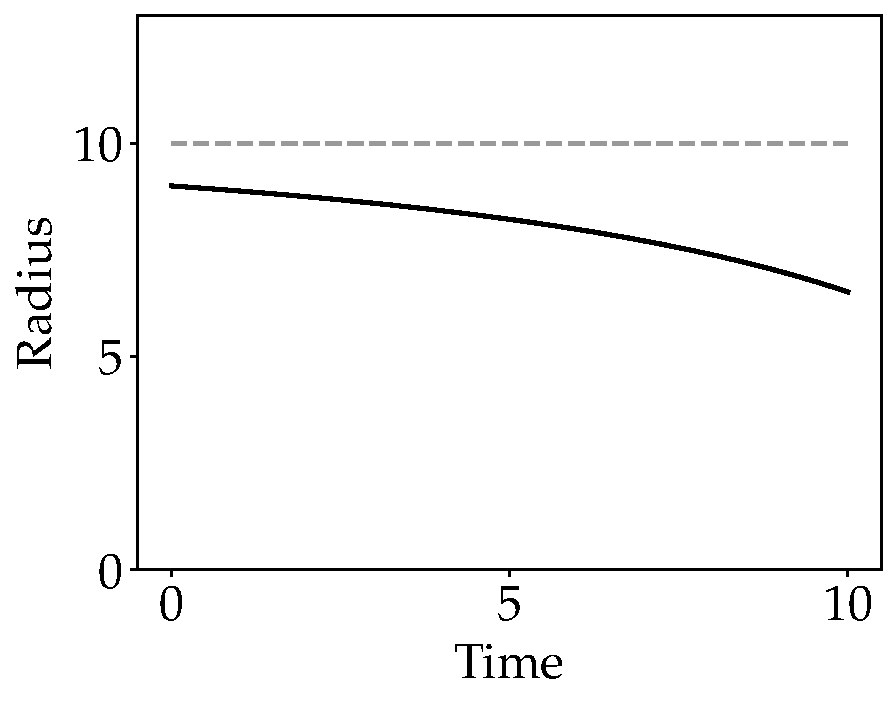
\includegraphics[width=0.85\linewidth]{solution_2}%
      \label{fig:solution:2}
    } \\
    \subfloat[$r_0 = 10, a = -1, b = 10$]{
      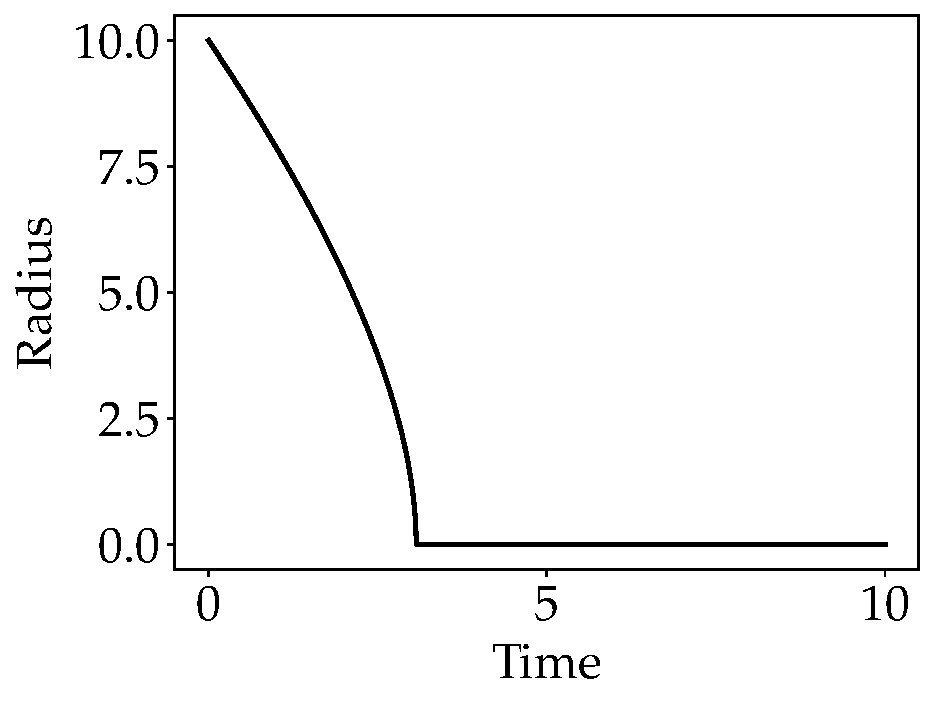
\includegraphics[width=0.85\linewidth]{solution_3}%
      \label{fig:solution:3}
    }
  \end{tabular}
  \caption{Solutions to the advection and mean curvature flow of a sphere. The three conditions correspond to (\ref{fig:solution:1}) growth, (\ref{fig:solution:2}) shrinking, and (\ref{fig:solution:1}) shrinking with negative advection. The dashed line denotes the meta-stable point.}
  \label{fig:solution}
\end{figure}

\section{Conclusion}
A closed-form solution for the motion of a sphere under advection and mean curvature flow is developed.
Vanishing times for the sphere are also calculated.
This model provides a closed-form solution for testing numerical solvers of advection and mean curvature flow and inverse problems therein.

% if have a single appendix:
%\appendix[Proof of the Zonklar Equations]
% or
%\appendix  % for no appendix heading
% do not use \section anymore after \appendix, only \section*
% is possibly needed

% use appendices with more than one appendix
% then use \section to start each appendix
% you must declare a \section before using any
% \subsection or using \label (\appendices by itself
% starts a section numbered zero.)
%


% \appendices


% \section{Python}
\appendices



\appendix[Source Code]
\label{app:python}
Source code is provided in Python for ease of implementation.

\lstdefinestyle{CustomStyle}{
  language=Python,
  numbers=none,
  stepnumber=1,
  numbersep=10pt,
  tabsize=4,
  showspaces=false,
  showstringspaces=false,
  breaklines=true
}
\lstset{basicstyle=\tiny,style=CustomStyle}
\lstinputlisting{./Figures/model.py}


% use section* for acknowledgment
% \section*{Acknowledgment}


% The authors would like to thank...


% Can use something like this to put references on a page
% by themselves when using endfloat and the captionsoff option.
\ifCLASSOPTIONcaptionsoff
  \newpage
\fi



% trigger a \newpage just before the given reference
% number - used to balance the columns on the last page
% adjust value as needed - may need to be readjusted if
% the document is modified later
%\IEEEtriggeratref{8}
% The "triggered" command can be changed if desired:
%\IEEEtriggercmd{\enlargethispage{-5in}}

% references section

\bibliographystyle{IEEEtran}
% argument is your BibTeX string definitions and bibliography database(s)
% \bibliography{,../bib/paper}
\bibliography{IEEEabrv,sphere.bib}


% can use a bibliography generated by BibTeX as a .bbl file
% BibTeX documentation can be easily obtained at:
% http://mirror.ctan.org/biblio/bibtex/contrib/doc/
% The IEEEtran BibTeX style support page is at:
% http://www.michaelshell.org/tex/ieeetran/bibtex/
%\bibliographystyle{IEEEtran}
% argument is your BibTeX string definitions and bibliography database(s)
%\bibliography{IEEEabrv,../bib/paper}
%
% <OR> manually copy in the resultant .bbl file
% set second argument of \begin to the number of references
% (used to reserve space for the reference number labels box)
% \begin{thebibliography}{1}

% \bibitem{IEEEhowto:kopka}
% H.~Kopka and P.~W. Daly, \emph{A Guide to \LaTeX}, 3rd~ed.\hskip 1em plus
%   0.5em minus 0.4em\relax Harlow, England: Addison-Wesley, 1999.

% \end{thebibliography}

% biography section
% 
% If you have an EPS/PDF photo (graphicx package needed) extra braces are
% needed around the contents of the optional argument to biography to prevent
% the LaTeX parser from getting confused when it sees the complicated
% \includegraphics command within an optional argument. (You could create
% your own custom macro containing the \includegraphics command to make things
% simpler here.)
%\begin{IEEEbiography}[{\includegraphics[width=1in,height=1.25in,clip,keepaspectratio]{mshell}}]{Michael Shell}
% or if you just want to reserve a space for a photo:



% You can push biographies down or up by placing
% a \vfill before or after them. The appropriate
% use of \vfill depends on what kind of text is
% on the last page and whether or not the columns
% are being equalized.

% Can be used to pull up biographies so that the bottom of the last one
% is flush with the other column.
%\enlargethispage{-5in}



% that's all folks
\end{document}
